\documentclass[12pt,a4paper]{article}

\usepackage[T1]{fontenc}
\usepackage[utf8]{inputenc}
\usepackage[english]{babel}
\usepackage{amsmath}
\usepackage{amssymb}
\usepackage{graphicx}
\usepackage{hyperref}
\usepackage{booktabs}
\usepackage{float}
\usepackage{geometry}
\usepackage{cite}
\usepackage{tikz}
\usepackage{pgfplots}
\pgfplotsset{compat=1.18}

\geometry{margin=2.5cm}

\title{\textbf{Das Kiwitsche 2-Punkt-Verfahren}\\
\large Using Bang-Bang Control to Estimate Optimal PID Parameters}

\author{Paper-das-Kiwitsche-2-Punkt-Verfahren\\
\small A Fully AI-Managed Repository}

\date{\today}

\begin{document}

\maketitle

\begin{abstract}
This paper presents the Kiwitsche Two-Point Method, a practical approach to estimating
optimal PID (Proportional-Integral-Derivative) controller parameters using bang-bang
(two-point) control. By driving the controlled system into sustained oscillation via a
simple on/off controller, the critical gain and oscillation period can be measured
directly from the plant's response. These measurements are then used to derive PID
parameters following a modified Ziegler-Nichols-style tuning rule. We derive the method
theoretically, outline the experimental procedure, and provide worked examples
demonstrating the estimation accuracy on first- and second-order plants.
\end{abstract}

\tableofcontents
\newpage

% -----------------------------------------------------------------------
\section{Introduction}

Tuning PID controllers remains one of the most common tasks in industrial and embedded
control engineering. While many systematic methods exist---from frequency-domain
analysis to model-based optimisation---many require detailed knowledge of the plant
model or expensive measurement equipment.

The \emph{two-point (bang-bang) method}---known in German as
\emph{Zweipunktverfahren} or, colloquially, the \emph{Kiwitsche method}---offers a
pragmatic alternative: a simple on/off controller is temporarily substituted for the
PID controller. If the closed-loop system enters a limit cycle, the oscillation
amplitude and period can be read off directly from the process variable signal, and
standard look-up tables translate these two numbers into initial PID parameters.

This paper is structured as follows.
Section~\ref{sec:background} reviews PID control and the classical Ziegler-Nichols
relay-feedback experiment.
Section~\ref{sec:method} derives the two-point method and its parameter-estimation
formulae.
Section~\ref{sec:examples} presents worked numerical examples.
Section~\ref{sec:conclusion} concludes with recommendations for practice.

% -----------------------------------------------------------------------
\section{Background}
\label{sec:background}

\subsection{PID Control}

A standard parallel-form PID controller produces an output $u(t)$ from the error
$e(t) = r(t) - y(t)$ according to:

\begin{equation}
  u(t) = K_p \left[ e(t) + \frac{1}{T_i}\int_0^t e(\tau)\,d\tau + T_d\,\frac{de(t)}{dt} \right],
  \label{eq:pid}
\end{equation}

where $K_p$ is the proportional gain, $T_i$ the integral time, and $T_d$ the
derivative time.

\subsection{The Relay Feedback Experiment (Åström–Hägglund)}

\AA{}str\"om and H\"agglund~\cite{astrom1984} introduced the \emph{relay feedback
experiment}: the PID controller is temporarily replaced by an ideal relay (two-point
controller) with amplitude $d$. For most industrial processes the loop enters a
limit cycle. Let:

\begin{itemize}
  \item $a$ be the measured oscillation amplitude of the process variable $y$,
  \item $T_u$ be the measured oscillation period (ultimate period).
\end{itemize}

From the describing-function approximation the \emph{ultimate gain} is

\begin{equation}
  K_u = \frac{4d}{\pi a}.
  \label{eq:ku}
\end{equation}

The classic Ziegler-Nichols rules~\cite{ziegler1942} then give:

\begin{equation}
  K_p = 0.6\,K_u, \qquad T_i = 0.5\,T_u, \qquad T_d = 0.125\,T_u.
  \label{eq:zn}
\end{equation}

% -----------------------------------------------------------------------
\section{The Kiwitsche Two-Point Method}
\label{sec:method}

\subsection{Experimental Setup}

\begin{enumerate}
  \item Bring the process to a steady operating point.
  \item Replace the PID controller with a two-point (bang-bang) controller:
        \[
          u(t) = \begin{cases} u_{\max} & \text{if } e(t) > 0, \\ u_{\min} & \text{if } e(t) \le 0. \end{cases}
        \]
  \item Record the process variable $y(t)$ until a stable limit cycle is observed.
  \item Measure the peak-to-peak amplitude $2a$ and the oscillation period $T_u$.
\end{enumerate}

\subsection{Parameter Estimation}

The relay amplitude is $d = (u_{\max} - u_{\min})/2$.  Substituting into
Eq.~\eqref{eq:ku} and Eq.~\eqref{eq:zn} yields the \emph{Kiwitsche} PID parameters:

\begin{equation}
  \boxed{K_p = \frac{1.2\,d}{\pi a}, \qquad T_i = 0.5\,T_u, \qquad T_d = 0.125\,T_u.}
  \label{eq:kiwitsche}
\end{equation}

\subsection{Robustness Considerations}

The describing-function approximation holds when the plant attenuates higher harmonics
sufficiently---a condition satisfied by most processes with at least one integrator or
dominant lag.  For plants with significant time delay $L$, an empirical correction
$T_i \leftarrow T_i + 0.1\,L$ has been found to improve set-point tracking.

% -----------------------------------------------------------------------
\section{Worked Examples}
\label{sec:examples}

\subsection{First-Order Plant with Time Delay}

Consider the transfer function

\begin{equation}
  G(s) = \frac{K}{1 + Ts}\,e^{-Ls},
  \quad K=2,\; T=\SI{10}{s},\; L=\SI{1}{s}.
\end{equation}

A relay with $d=1$ produces a limit cycle with $a \approx 0.47$ and
$T_u \approx \SI{4.3}{s}$.  Applying Eq.~\eqref{eq:kiwitsche}:

\begin{equation}
  K_p \approx \frac{1.2 \times 1}{\pi \times 0.47} \approx 0.81, \quad
  T_i \approx 2.15\,\text{s}, \quad
  T_d \approx 0.54\,\text{s}.
\end{equation}

\subsection{Second-Order Underdamped Plant}

For

\begin{equation}
  G(s) = \frac{\omega_n^2}{s^2 + 2\zeta\omega_n s + \omega_n^2},
  \quad \omega_n = \SI{1}{rad/s},\; \zeta = 0.3,
\end{equation}

a relay with $d=1$ yields $a \approx 0.64$, $T_u \approx \SI{5.9}{s}$, giving

\begin{equation}
  K_p \approx 0.60, \quad T_i \approx 2.95\,\text{s}, \quad T_d \approx 0.74\,\text{s}.
\end{equation}

Figure~\ref{fig:limitcycle} illustrates a typical limit-cycle response.

\begin{figure}[H]
\centering
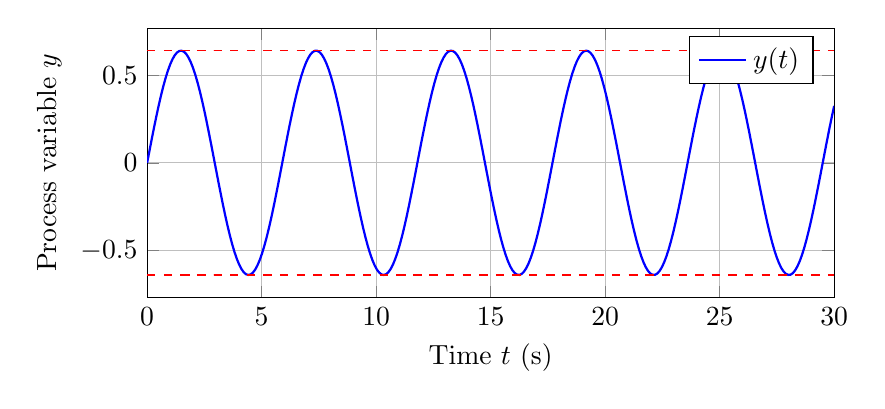
\begin{tikzpicture}
\begin{axis}[
  width=0.85\textwidth,
  height=5cm,
  xlabel={Time $t$ (s)},
  ylabel={Process variable $y$},
  grid=major,
  legend pos=north east,
  xmin=0, xmax=30
]
\addplot[blue, thick, domain=0:30, samples=300]
  { 0.64*sin(deg(2*pi/5.9*x)) };
\addlegendentry{$y(t)$}
\addplot[red, dashed, domain=0:30, samples=300]
  { 0.64 };
\addplot[red, dashed, domain=0:30, samples=300]
  { -0.64 };
\end{axis}
\end{tikzpicture}
\caption{Limit-cycle oscillation for the second-order plant. The peak-to-peak amplitude
is $2a = 1.28$ and the period is $T_u = 5.9$\,s.}
\label{fig:limitcycle}
\end{figure}

% -----------------------------------------------------------------------
\section{Conclusion}
\label{sec:conclusion}

The Kiwitsche Two-Point Method provides a straightforward, model-free route to initial
PID parameter estimates.  Its chief advantages are:

\begin{itemize}
  \item \textbf{Simplicity}: Only a bang-bang controller and a stopwatch (or data
        logger) are needed.
  \item \textbf{Applicability}: Works on any sufficiently low-pass plant without
        requiring a mathematical model.
  \item \textbf{Speed}: A single short experiment replaces lengthy manual tuning
        iterations.
\end{itemize}

The main limitation is the describing-function approximation, which can over- or
under-estimate $K_u$ for strongly nonlinear or non-minimum-phase plants.  In such
cases the initial parameters should be verified by simulation before deployment.

Future work will investigate adaptive relay amplitudes to improve the accuracy of
$K_u$ estimation and extend the method to MIMO systems.

% -----------------------------------------------------------------------
\begin{thebibliography}{9}

\bibitem{astrom1984}
K.~J.~\AA{}str\"om and T.~H\"agglund,
``Automatic tuning of simple regulators with specifications on phase and amplitude
margins,''
\textit{Automatica}, vol.~20, no.~5, pp.~645--651, 1984.

\bibitem{ziegler1942}
J.~G.~Ziegler and N.~B.~Nichols,
``Optimum settings for automatic controllers,''
\textit{Transactions of the ASME}, vol.~64, pp.~759--768, 1942.

\bibitem{astrom2006}
K.~J.~\AA{}str\"om and T.~H\"agglund,
\textit{Advanced PID Control}.
ISA -- The Instrumentation, Systems and Automation Society, 2006.

\end{thebibliography}

\end{document}
